\newpage
\section{Подсистема справочников}

Подсистема справочников предоставляет инструменты для ведения единых справочников, которые совместно используются  ФТМИС и интегрируемыми подсистемами.

При переходе в подсистему справочников открывается главная страница подсистемы (Рисунок \ref{img_spr_main}). В верхней части страницы расположены наименования групп справочников. Для перехода к работе с определенным справочником необходимо щелкнуть левой кнопкой мыши по названию группы, а затем, в появившемся меню выбрать наименование справочника. Доступ к основным справочникам системы можно получить, нажав на соответствующую кнопку на главной странице подсистемы.

\begin{figure}[ht]\centering
 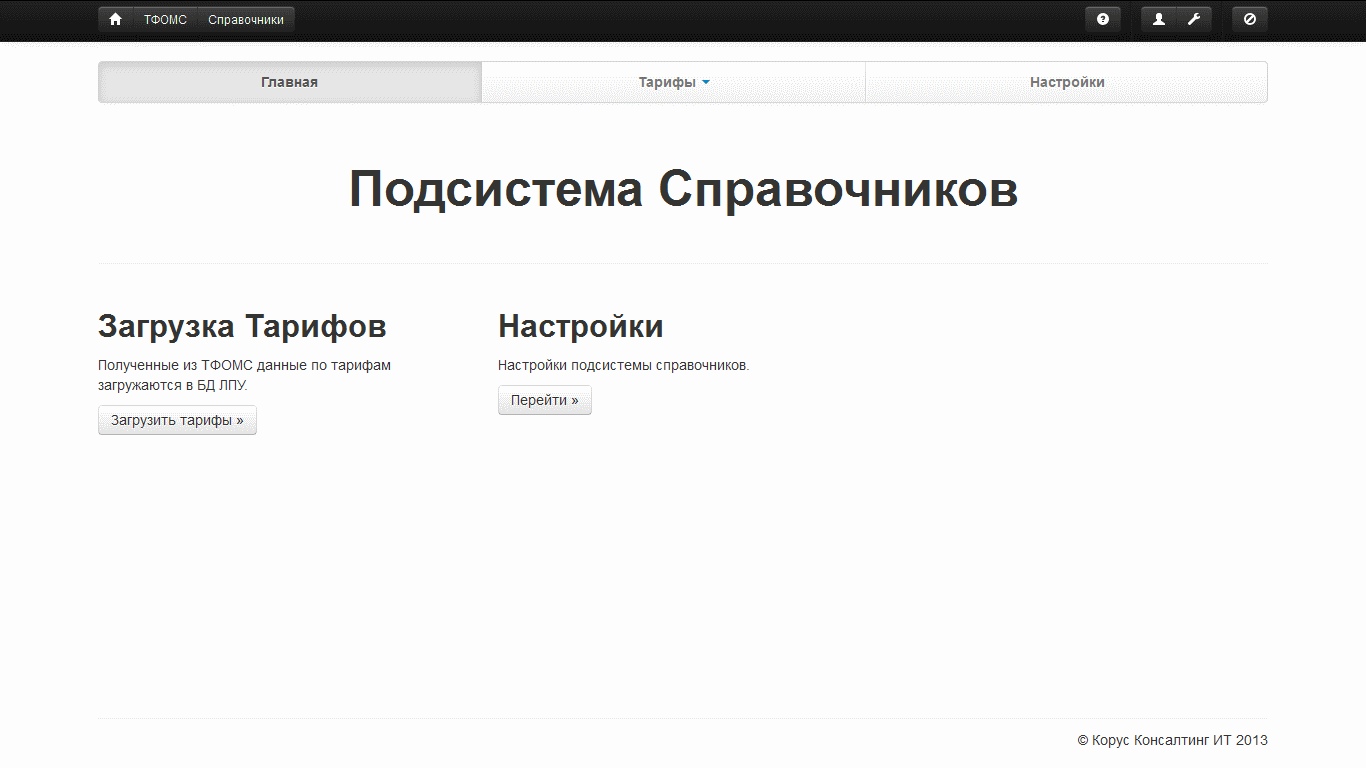
\includegraphics[width = 1\textwidth ,keepaspectratio]{spr_main}
 \caption{Главная страница подсистемы справочников}
 \label{img_spr_main}
\end{figure}

\subsection{Загрузка тарифов}

В данном разделе подсистемы осуществляется загрузка справочника тарифов по оплате услуг ЛПУ.

Для перехода в данный раздел (Рисунок \ref{img_spr_load}) необходимо нажать кнопку \btn{Тарифы}  в верхней части любой страницы подсистемы и в появившемся меню выбрать пункт Загрузка, либо нажать кнопку \btn{Загрузить тарифы >>} на главной странице подсистемы.

\begin{figure}[ht]\centering
 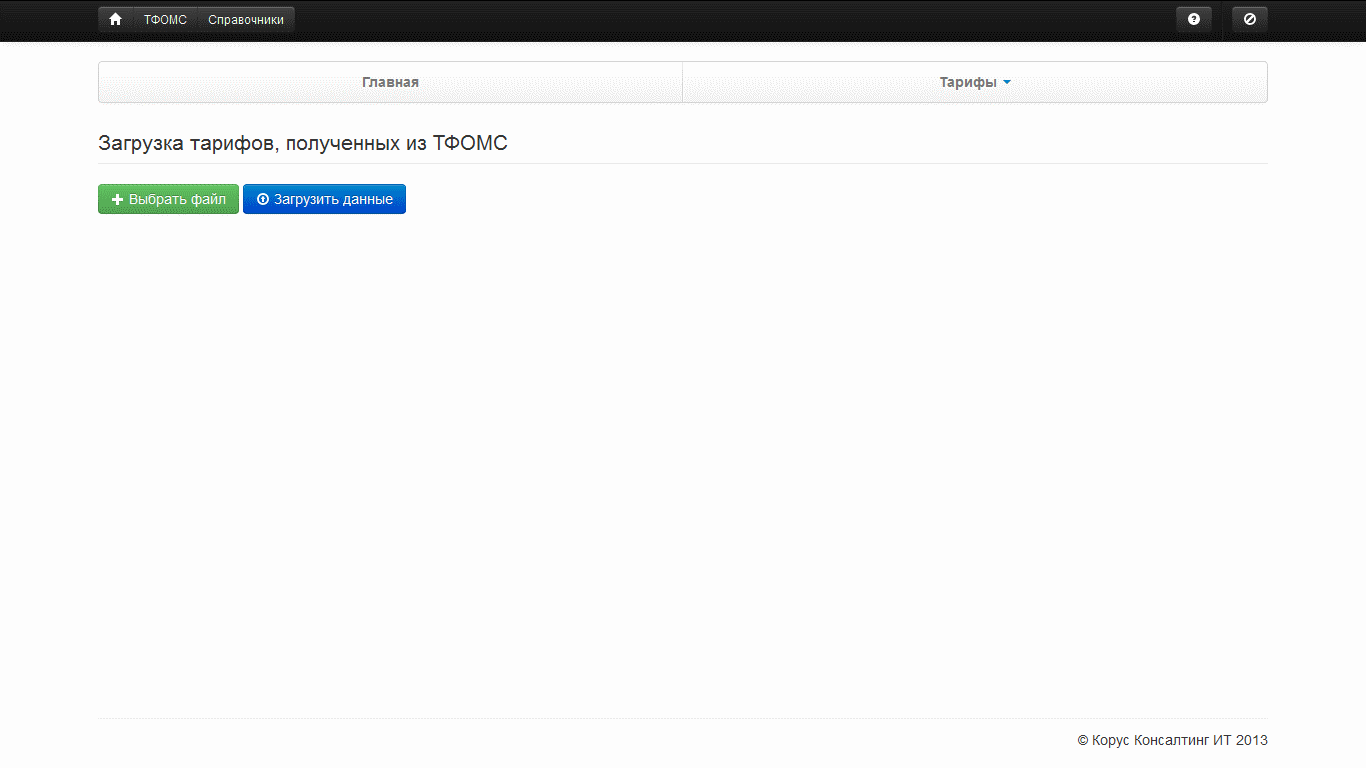
\includegraphics[width = 1\textwidth ,keepaspectratio]{spr_load}
 \caption{Страница загрузки справочника тарифов}
 \label{img_spr_load}
\end{figure}

Для загрузки тарифов необходимо нажать на кнопку \btn{Выбрать файл}, в открывшемся окне перейти в нужную папку и выбрать файл для загрузки. После выбора файла его имя появится под кнопкой \btn{Выбрать файл}. Далее необходимо нажать кнопку  \btn{Загрузить данные}. После некоторого времени ожидания на странице появится сообщение о результатах загрузки (Рисунок \ref{img_spr_load_rez}).

\begin{figure}[ht]\centering
 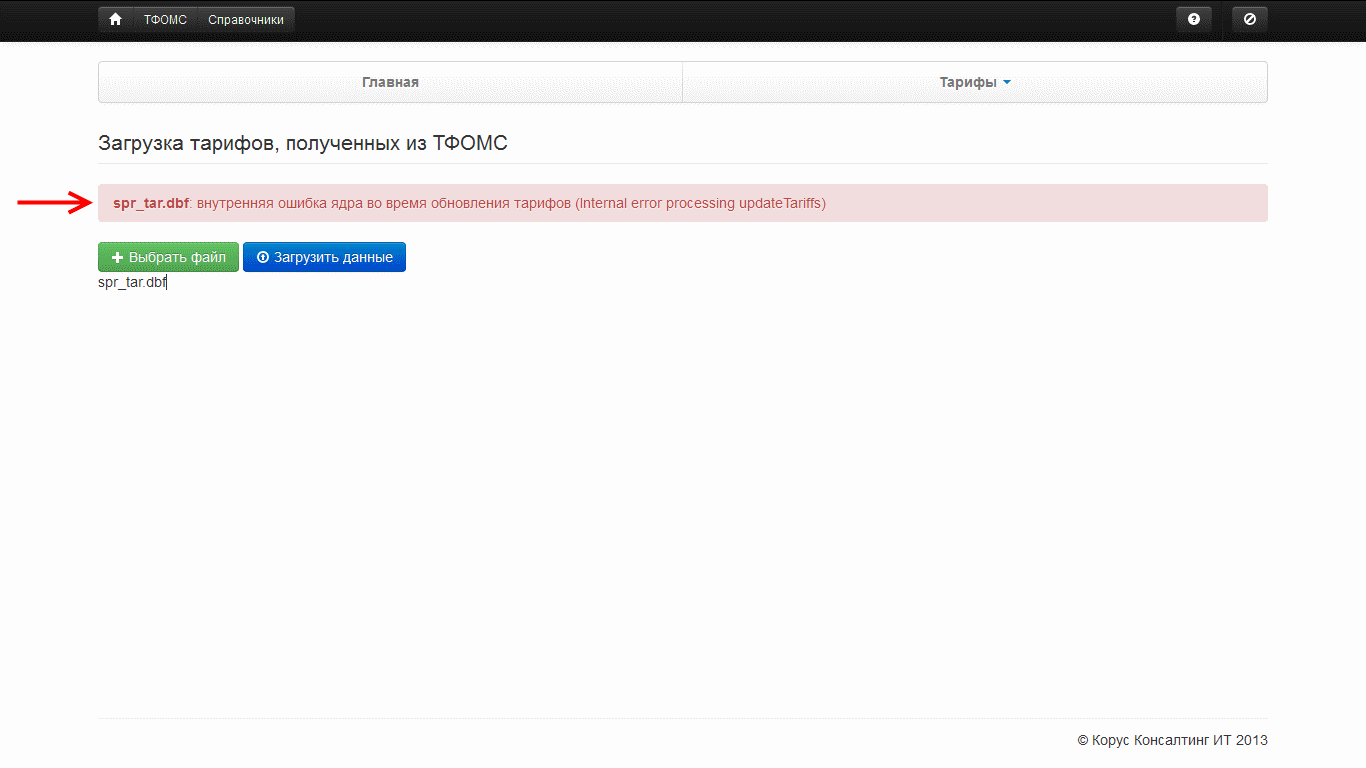
\includegraphics[width = 1\textwidth ,keepaspectratio]{spr_load_rez}
 \caption{Результат загрузки тарифов}
 \label{img_spr_load_rez}
\end{figure}